\section[Unsupervised ML]{Unsupervised machine learning}

\begin{frame}{A lot of applications and use cases, \ldots}
\ldots but we'll distinguish two today:

\begin{enumerate}
\item Finding similar variables (dimension reduction)
\item Finding similar cases (clustering)
\end{enumerate}

\pause

Are we more interested in which features ``belong together'' or which cases ``belong together''? 

\emph{There are many other techniques than those presented today, and vice versa, those presented today can also be used for other purposes}

\end{frame}

\subsection{Finding similar variables}

\subsubsection{An introduction to dimensionality reduction}


\begin{frame}{Dimensionality reduction}
dimensionality = the number of features we have
\begin{block}{(1) Explorative data analysis and visualization}
\begin{itemize}
\item No good way to visualize 10,000 dimensions (or even 4)
\end{itemize}
\end{block}

\pause

\begin{block}{(2) The curse of dimensionality}
More features means more data (good!), but:
\begin{itemize}
\item Too many features can lead to unfeasible computation times
\item We need more training cases to increase the likelihood that the possible combinations actually occur
\end{itemize}
\end{block}
\end{frame}



\begin{frame}[fragile]{Dimensionality reduction}

\begin{block}{Feature extraction}
\begin{itemize}
\item Create a smaller set of features
\item E.g.: 1,000 features $\rightarrow$ PCA to reduce to 50 components $\rightarrow$ SML with these 50 component scores as features
\end{itemize}
\end{block}

\end{frame}



\begin{frame}[fragile]{Dimensionality reduction}

So, we can use unsupervised ML as a dimension reduction step in a supervised ML pipeline. 
\vspace{0.5cm}

But it can also be a goal in itself, to understand the data better or to visualize them.
\end{frame}







\subsubsection{Principal Component Analysis and Singular Value Decomposition}


\begin{frame}{PCA}
\begin{itemize}
\item related to and often confused with Factor Analysis (same menu item in SPSS -- many people who believe they run FA actually run PCA!)
\item Components are ordered (first explains most variance)
\item Components do \emph{not} necessarily carry a meaningful interpretation
\end{itemize}
\end{frame}

\begin{frame}{PCA}
\makebox[\linewidth]{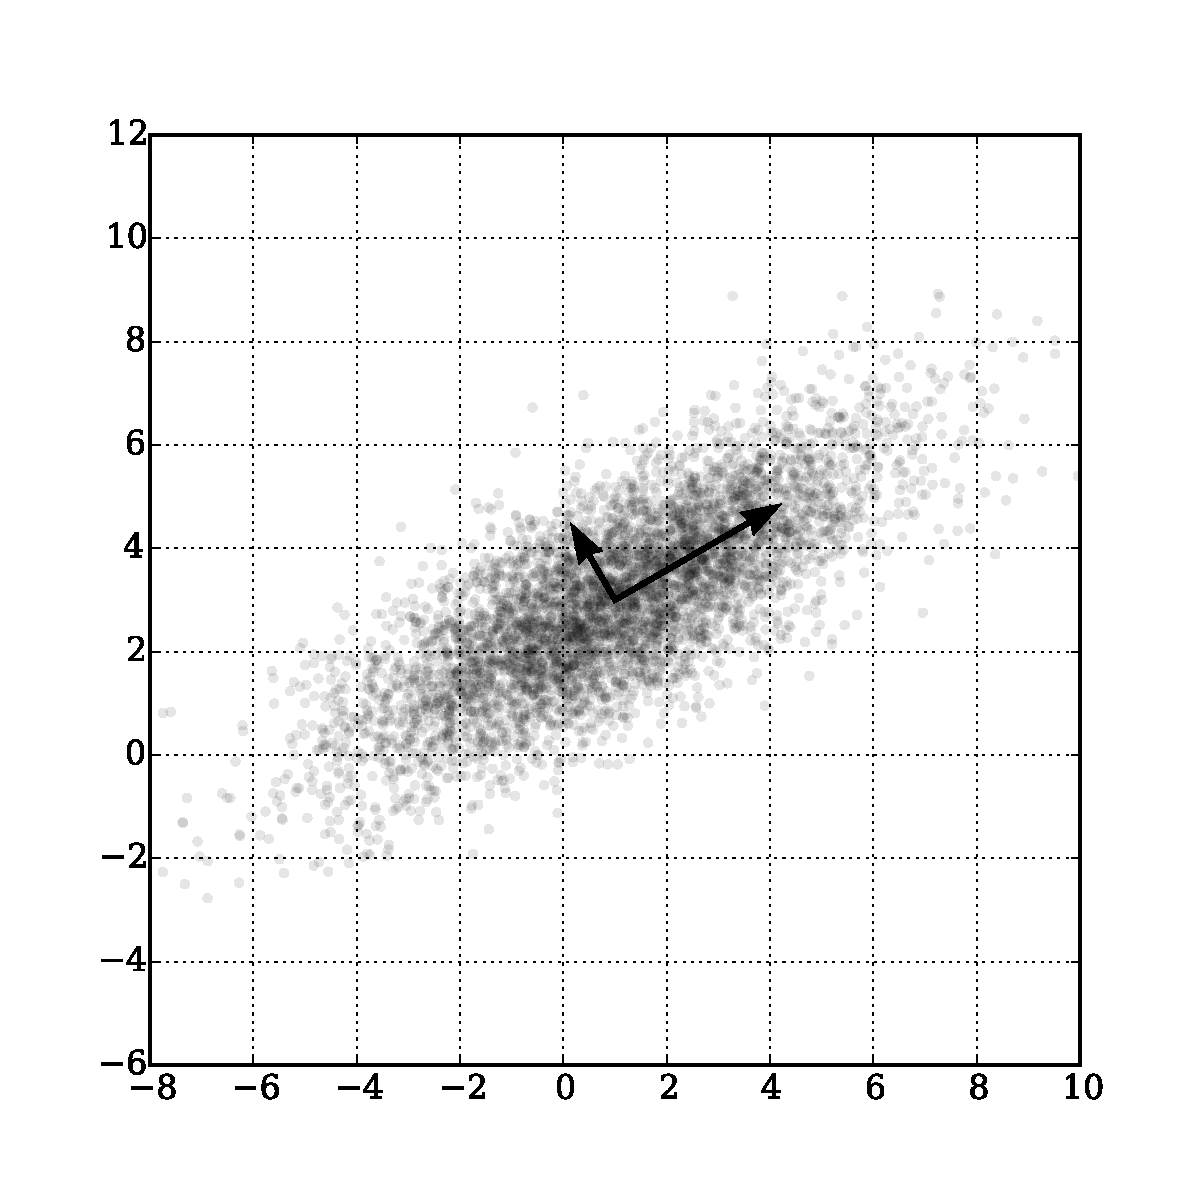
\includegraphics[width=\paperwidth,height=.6\paperheight,keepaspectratio]{pca}}

\tiny{\url{https://upload.wikimedia.org/wikipedia/commons/f/f5/GaussianScatterPCA.svg}}
\end{frame}



\begin{frame}[fragile,plain]{Preparation: Import modules and get some sample data}
\begin{minted}{python}
import pandas as pd
from sklearn.decomposition import PCA
from sklearn.preprocessing import StandardScaler

df = pd.read_csv("https://cssbook.net/d/eurobarom_nov_2017.csv")\
    .dropna()\
    .groupby(["country"])[[
    "support_refugees_n", 
    "support_migrants_n", 
    "age", 
    "educational_n"]].mean()
\end{minted}


\begin{lstlistingoutputtiny}
country   support_refugees_n  support_migrants_n        age  educational_n                                                                
Austria             2.847674            2.576744  49.445349      18.930233
Belgium             2.772619            2.252381  53.002381      19.338095
Bulgaria            2.075159            1.769427  51.517197      19.652229
Croatia             2.717105            2.002193  47.001096      18.899123
Cyprus              3.018141            2.104308  53.734694      18.598639
\end{lstlistingoutputtiny}
\end{frame}






\begin{frame}[fragile,plain]{Running PCA}
  \begin{minted}{python}
# we first standardize our data to z-scores
scaler = StandardScaler()
df_s = scaler.fit_transform(df) 
    
mypca = PCA()
componentscores = mypca.fit_transform(df_s)
scores_df = pd.DataFrame(componentscores, index=df.index)

components_df = pd.DataFrame(data=mypca.components_.T)
components_df.index = df.columns
print("Variable loadings on the 4 components:")
print(components_df)  

# This is the transformed dataset
# As we will see in a minute, we retain 86\% of the
# variance even if we keep only the first 2 components
print("The component scores for each case:")
print(scores_df)
\end{minted}
\end{frame}



\begin{frame}[fragile,plain]{Running PCA}
\begin{lstlistingoutputtiny}
Variable loadings on the 4 components:
                           0         1         2         3
support_refugees_n  0.573292 -0.369010  0.139859  0.718058
support_migrants_n  0.513586 -0.533140 -0.094283 -0.665659
age                 0.445117  0.558601  0.670994 -0.199005
educational_n       0.457642  0.517261 -0.722023  0.041073


The component scores for each country:
                       0         1         2         3
country                                               
Austria        -0.103285 -1.220018 -0.535673  0.066888
Belgium        -0.029355 -0.084707  0.051515  0.227609
Bulgaria       -1.660518  0.949533 -0.480337 -0.151837
Croatia        -1.267502 -0.819093 -0.920657  0.843682
Cyprus          0.060590 -0.195928  0.573670  0.812519
Czech republic -2.219795  0.675655 -0.763679 -0.086147
Denmark         2.925631  1.516636 -0.748940  0.495489
Estonia        -0.602217  2.206418  0.785869 -0.152262
Finland         2.224310  1.384983 -0.169499 -0.468742
France         -0.102062 -0.046415  0.228587 -0.122965
Germany         0.917864 -0.259560  0.940792  0.319158
Greece         -0.832343 -0.313480  0.329525  0.683748
Hungary        -2.234701  0.716823  0.391788 -0.315312
Ireland         0.993243 -1.767147 -0.592957 -0.168892
\end{lstlistingoutputtiny}
\end{frame}









\begin{frame}[fragile,plain]{Plotting the result}
  \begin{minted}{python}
import bioinfokit.visuz
   
bioinfokit.visuz.cluster.biplot(cscore=componentscores, 
  loadings=mypca.components_, 
  labels=df.columns, 
  var1=round(mypca.explained_variance_ratio_[0],2), 
  var2=round(mypca.explained_variance_ratio_[1],2), 
  show=True)  
\end{minted}

\makebox[\linewidth]{\includegraphics[width=\paperwidth,height=.6\paperheight,keepaspectratio]{pca-example-book}}

\end{frame}



\begin{frame}[fragile,plain]{Plotting the result}
  \begin{minted}{python}
import numpy as np
import matplotlib.pyplot as plt

fig, ax = plt.subplots()
ax.plot(np.cumsum(mypca.explained_variance_ratio_))
ax.set_xticks(range(mypca.n_components_))
ax.set_xticklabels(range(1, mypca.n_components_+1))
ax.set_xlabel("number of components") 
ax.set_ylabel("cumulative explained variance") 
ax.set_ylim(0,1)
fig.savefig("pca-explained-variance.png")   # optional of course
\end{minted}

\makebox[\linewidth]{\includegraphics[width=\paperwidth,height=.3\paperheight,keepaspectratio]{pca-explained-variance}}

\end{frame}






\begin{frame}{Singular value decomposition}

\begin{alertblock}{PCA uses a dense matrix!}
In ``real life'' with larger datasets (essentially, everything (!) involving text), we never use PCA but SVD. It works exactly the same (check out \url{scikit-learn.org}), but does not require to hold a dense matrix in memory. Instead, it operates on a sparse matrix, in which only non-zero values are stored. (this will make a lot of sense once we talk about textual data)
\end{alertblock}

  
\footnotesize{
* It's mathematically different, but SVD is even used ``under the hood'' by several PCA modules to solve PCA problems.
More info and background: \url{https://towardsdatascience.com/pca-and-svd-explained-with-numpy-5d13b0d2a4d8}}
\end{frame}







\subsection{Finding similar cases}

\subsubsection{k-means clustering}

\begin{frame}{Grouping features vs grouping cases}
  \begin{itemize}[<+->]
  \item  In the previous example, we established that \emph{age} and \emph{education} measure almost the same thing, and so do \emph{support\_refugees} and \emph{support\_migrants}.
  \item We could now, for instance, check out which countries receive similar scores to group them.
  \item But if grouping countries (instead of variables) is our goal in the first place, we can directly do so.
  \end{itemize}
\end{frame}




\begin{frame}{k-means clustering}
\begin{itemize}[<+->]
\item Goal: group cases into $k$ clusters
\item $k$ is set in advance
\item Algorithm to determine \textit{k} centroids (points in the middle of the cases that belong to it) such that the distances between the cases and their centroids are minimized
\item non-deterministic: starts with a randomly choosen centroids (there are other versions)
\item Cheap to compute: works even with large number of cases
\item We can run PCA first to reduce the number of features if we want/need to
\end{itemize}
\end{frame}




\begin{frame}{k-means clustering}
\makebox[\linewidth]{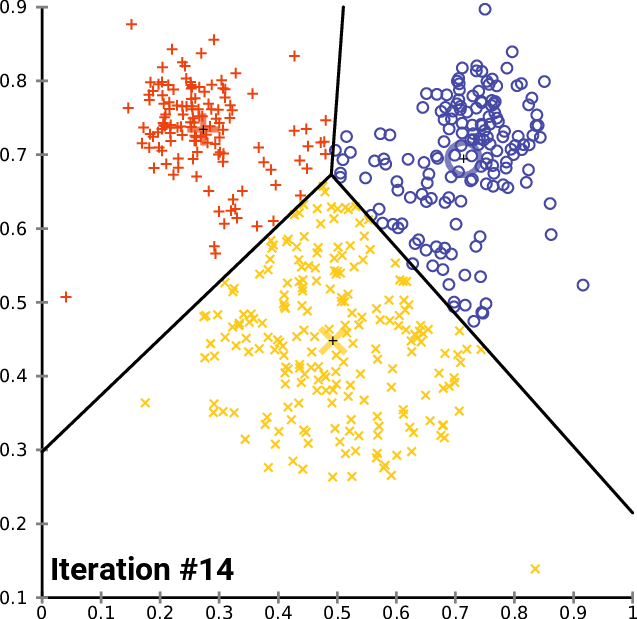
\includegraphics[width=\paperwidth,height=.65\paperheight,keepaspectratio]{kmeans}}

{\tiny{\url{https://upload.wikimedia.org/wikipedia/commons/e/ea/K-means\_convergence.gif}}}

Notice the big symbols indicating the centroids.
\end{frame}


\begin{frame}[plain,fragile]
\begin{lstlisting}
from sklearn.cluster import KMeans

# everything needs to be measured on the same scale,
# therefore we take the scaled dataset

mykm = KMeans(n_clusters=3).fit(df_s)
pd.DataFrame({"country":df.index, "cluster":mykm.labels_})
\end{lstlisting}

\begin{lstlistingoutputtiny}
           country  cluster
0          Austria        1
1          Belgium        1
2         Bulgaria        0
3          Croatia        0
4           Cyprus        1
5   Czech republic        0
\end{lstlistingoutputtiny}

\end{frame}



\begin{frame}{Finding the optimal $k$}

\begin{itemize}
\item The only way to find $k$ is to estimate multiple models with different $k$s
\item No single best solution; finding a balance between error within clusters (distances from centroid) and low number of clusters.
\item An elbow plot can be helpful
\end{itemize}
\end{frame}


\begin{frame}[fragile,plain]{Finding the optimal $k$}
\begin{minted}{python}
wss = []
for i in range(1, 15):
    km = KMeans(n_clusters=i)
    km.fit(df_s)
    wss.append(km.inertia_)

fig, ax = plt.subplots()
ax.plot(range(1, 15), wss, marker="o")
ax.set_xlabel("Number of clusters")
ax.set_ylabel("Within groups sum of squares")
\end{minted}

\makebox[\linewidth]{\includegraphics[width=\paperwidth,height=.3\paperheight,keepaspectratio]{kmeans-elbow}}

\end{frame}





\subsubsection{Hierarchical clustering}

\begin{frame}{Downsides of k-means clustering}
k-means is fast, but has problems:

\begin{itemize}
\item $k$ can only be determined by fitting multiple models and comparing them
\item bad results if the wrong $k$ is chosen
\item bad results if the (real) clusters are non-spherical
\item bad results if the (real) clusters are not evenly sized
\end{itemize}
\end{frame}


\begin{frame}{Hiearchical clusttering}
\begin{block}{General idea}
\begin{itemize}
\item To start, each case has its own cluster
\item Merge the two clusters that are most similar
\item Repeat until desired number of clusters is reached
\end{itemize}

\end{block}

\pause

\begin{block}{Different options}
\begin{itemize}
\item Stopping criterion: based on numerical statistic (e.g., Duda-Hart) or dendrogram
\item Linkage: how to determine which two clusters should be merged?
\end{itemize}

\end{block}
\end{frame}


\begin{frame}{Let's look into some options}

\url{https://scikit-learn.org/stable/modules/clustering.html\#hierarchical-clustering}

$\Rightarrow$ Ward's linkage is a good default all-rounder choice, especially if you encounter the problem that other linkages lead to almost all cases ending up in one cluster. 
\end{frame}


\begin{frame}{Hierarchical clustering takeaway}
\begin{itemize}
\item The main reason \emph{not} to use hierarchical methods (but k-means) is their computational cost: when clustering survey data of media users, never use $k$-means!
\item But for NLP/ML, costs may be too high (if not used carefully)
\item Very much worth considering, though, if you are really into grouping cases!
\end{itemize}
\end{frame}


\begin{frame}{Important notes (for \emph{all} techniques today)}
\begin{block}{Consider the scales of measurement}
Clustering is based on distances -- if your features are not measured on the same scale, or if it is not meaningful to calculate a numerical distance, it won't produce meaningful results!

Consider standardizing/whitening your features!
\end{block}

\pause

\begin{block}{Pay attention outliers/extreme cases}
Extreme cases or outliers can have a strong influence.
\end{block}

\pause 
\begin{block}{Do proper pre-processing}
To reduce the number of features, but also to have \emph{meaningful} features (dimensions on which you expect high distances between the clusters).
\end{block}


\end{frame}




